\documentclass{article}

% IMPORT PACKAGES
\usepackage{graphicx}
\graphicspath{{images/}}
\usepackage{blindtext}
\usepackage[T1]{fontenc}
\usepackage[latin9]{inputenc}
\usepackage[a4paper]{geometry}
\geometry{verbose,tmargin=2cm,bmargin=2cm,lmargin=1cm,rmargin=1cm}
\setlength{\parskip}{\smallskipamount}
\setlength{\parindent}{0pt}
\usepackage{array}
\usepackage{mathtools}
\usepackage{dsfont}
\usepackage{amsmath}
\usepackage{amssymb}
\usepackage{lmodern}
\usepackage{eqlist}
\usepackage{babel}
\usepackage{multicol}
\usepackage{stackengine}
\usepackage{xcolor}
\usepackage{listings}
% BLOCKS
\usepackage{beamerarticle}
\usepackage[most]{tcolorbox}
%	COMMON COLORS
\definecolor{_light_green}{rgb}{0.36, 0.84, 0.36}
\definecolor{_light_grey}{rgb}{0.90, 0.90, 0.90}
\definecolor{_white}{rgb}{1.0, 1.0, 1.0}
\definecolor{_blue}{rgb}{0.0, 0.0, 1.0}
\definecolor{_light_blue}{rgb}{0.7, 0.9, 1.0}
%	DEFINE BOXES
\newtcolorbox{_block}[1][]{
    colbacktitle=_light_grey,		% title background
    coltitle=black,					% title color
    titlerule=0pt,
    colback=white!50!_light_grey,	% body background
    boxrule=0.4pt,					% content-frame padding (or frame width)
    colframe=black!20!_light_grey,	% frame color
    left=0mm,						% content and title left padding
    arc=0.5pt,						% border-radius
    title={#1},
}
\newtcolorbox{_example}[1][]{
    colbacktitle=_light_green,
    coltitle=black,
    titlerule=0pt,
    colback=white!60!_light_green,
    boxrule=0pt,
    colframe=white,
    left=0mm,
    arc=0.5pt,
    title={#1},
}
\newtcolorbox{_note}[1][]{
    colbacktitle=_light_blue,
    coltitle=black,
    titlerule=0pt,
    colback=white!60!_light_blue,
    boxrule=0pt,
    colframe=white,
    left=0mm,
    arc=0.5pt,
    title={#1},
}
\newtcolorbox{_block_emph}[1][]{
    enhanced,
    frame hidden,
    borderline west={2.0pt}{0pt}{blue!60!white},
    opacityframe=0.0,
    colback=blue!4!white,
    left=2mm,
    arc=0.5pt,
    title={#1},
}
%   CUSTOM CODE LISTINGS
\newtcblisting{code}[2][]{
	colback=blue!5!white,
	colframe=red!75!black,
	opacityframe=0.0,
	coltitle=black,
	left=5pt,
	lefttitle=0pt,
	enhanced,
	listing only,
	title=\textbf{#2},
	arc=0.5pt,
	listing engine=minted,
	minted language={#1},
	minted style=colorful,
	minted options={
		fontfamily=\sfdefault,%\sserif
		fontsize=\scriptsize,
		breaklines,
		autogobble, %linenos, %numbersep=1mm,
		tabsize=4,
		escapeinside=||,mathescape=true,
	},
	overlay={
		\begin{tcbclipinterior}
			\fill[black!30!white] (frame.south west) 
			rectangle ([xshift=1mm]frame.north west);
		\end{tcbclipinterior}
	},
}

% below command to set inline code style doesn't work    :(
\lstset{language=C,keywordstyle={\bfseries \color{blue}}}

% \usepackage{subfiles}
% \subfile{}

% DOCUMENT

\begin{document}

% short title:
%   \part*{}
%   \part[]{}

\title{CS4223 Project 2\\Cache Simulator}
\author{Justin Lu, Leon Thomm}
\maketitle

% changing sections enumeration style
% styles: \arabic{} \alph{} \Alph{} \roman{} \Roman{}
\renewcommand\thesection{\arabic{section}}
\renewcommand\thesubsection{\thesection.\alph{subsection}}

\section{Abstract}

\section{Specifications}

\begin{multicols}{2}

\textbf{processor behavior}

\begin{itemize}
    \item A processor executes instructions on every clock tick; if there's memory access it calls the cache and idles until it receives a response. (*)
\end{itemize}

\textbf{bus behavior}

\begin{itemize}
    \item A cache communicates with other caches through the bus, and the bus is "owned" (locked) by a cache until it completely finished his transactions corresponding to one transition in the respective state diagram.
    \item Bus locking must be fair between the caches (request queue-style).
    \item The time for sending a bus transaction (address and transaction code) to other caches takes 2 cycles - just as long as sending only an address.
    \item All queued bus signals are always transmitted before a cache can lock the bus again - this ensures consistency.
\end{itemize}

\textbf{cache behavior}

\begin{itemize}
    \item Any cache can always immediately respond to bus requests (*). If the cache gets asked to deliver a block which is pending eviction, the block is assumed to be invalid and cannot be delivered anymore.
    \item While the penalty for loading a cache line from memory is 100 cycles, the MESI cache implements Illinois and thus first tries to get the line from another cache, which adds to these 100 cycles if no one has it.
    \item The system always prefers cache-to-cache transfer.
\end{itemize}

A snooping cache can receive bus signals triggering three kinds of actions (and any combinations)
    1. the cache responding / possibly providing some data
    2. a transition in the data cache
    3. bus signals as a result of (2)

We assume that action (1) can always be executed immediately, (notice the cache currently doesn't own the bus, because the cache who asked is owning it). However, the actual data cache might be busy resolving a request from the processor, so actions (2) and (3) must be buffered and handled later. Since the incoming bus signal should only have an effect on \textit{future} operations in the cache (and not on the one currently running), it is safe for the cache to handle the bus signal immediately \textit{after} completing the current processor request.

\textbf{further system and timing specs}

\begin{itemize}
    \item If cache $C_0$ tries to cache a block $b$, the action of asking other caches whether they have $b$, and the action of sending the bus signal resulting from the following transition in $C_0$ are two separate steps which both require bus communication; i.e. we ignore the fact that the other caches could theoretically infer some of these bus transactions from $C_0$'s asking.
    \item Arbitration policy: the processor/cache with lower id is preferred; e.g. if $P_0$ and $P_1$ want to write to the same block in the same cycle, $P_0$ will proceed and $P_1$ will have to adapt if necessary
    \item If multiple caches could deliver a line, there is no additional time needed to select one - the selection algorithm is expected to terminate in the same cycle.
    \item The memory is word-addressable not, byte-addressable.
    \item Memory is generally only updated on eviction/flushing. Dragon never explicitly updates memory, the memory is assumed to snoop \textit{BusUpd} signals.
    \item The caches do not flush their dirty lines at the end of the simulation.
    \item The simulation ends when all processors entered state \textit{Done} and and the bus is idling (finished sending any pending signals).
\end{itemize}

(*) as stated in the task description

\textbf{key insights}

\begin{enumerate}
    \item The bus can only do one thing at a time, it serializes all requests.
    \item All memory transfer goes through the bus.
    \item There are two types of signals a cache can receive: \textit{processor signals} and \textit{bus signals}.
    \item Each of these can be further divided into
        \begin{itemize}
            \item those that can be answered right away
            \item those that require communication with other caches or possibly memory
        \end{itemize}
\end{enumerate}

$\implies$ Let $C_0$ be a cache processing a processor request on address $a$ in block $b$ requiring communication over the bus, and assume $C_0$ is owning the bus now and performing its operations. Let $C_1$ be another cache attempting a state transition on $b$ as well. By owning the bus, $C_0$ ensures the following

\begin{itemize}
    \item \textbf{either} $C_1$ is blocked from its transition (if it requires sending \textbf{and receiving} on bus) until $C_0$ is done and the system never enters an invalid state because the bus distributes the necessary signals before $C_1$ can lock it
    \item \textbf{or} $C_1$'s transition does not require bidirectional communication on the bus (i.e. only sending a bus signal, e.g. MESI Invalid PrWrMiss) which might put the system into a temporarily invalid state (e.g. $b$ in Modified in $C_0$ and $C_1$) but this inconsistency will be serially resolved once $C_0$ is done, for the same reason as above
\end{itemize}

From the perspective of some cache $C_i$, the bus can be:

\begin{itemize}
    \item owned: $C_i$ can send bus requests
    \item foreign owned: $C_i$ can respond to incoming bus requests - owner is responsible of preventing conflicts
    \item busy: the bus is not owned by anyone but busy sending signals
    \item free: $C_i$ can try to acquire the bus lock in order to start sending requests
\end{itemize}

\end{multicols}

\section{Implementation}

\subsection{Approach 1 - Python Prototype}

\begin{multicols}{2}

We first wrote a prototype in Python to implement most of the basic concepts and gain an understanding of the challenges. This prototype works mainly by determining the number of cycles any operation will take as early as possible, and optimizes by simulating multiple cycles at once when it is safe to do so. The source code can be found on github in the \textit{cachesim-py} directory. Notice that this implementation does not yet fully follow the above specifications.

\subsection{Approach 2 - High Performance in Rust}

In attempt to come up with a more scalable design, we spent \textit{a lot} of time implementing a completely different solution in Rust. We chose Rust mainly for performance reasons and its design principles. Generally, a Rust implementation without any \textit{unsafe} code compiling is an extremely good indicator for the quality and stability of the written code. It can still fail, but when it does it's much more clear why and where, and most of typical sources for errors are already eliminated by the rules enforced by the compiler. Implementing the cache simulator in Rust We saw as a challenge and opportunity to try get more familiar with the language.

\subsubsection{order of execution}

Any simulator will have to step through a series of simulated cycles. A new cycles's rising edge (referred to as \textit{tick} from now on) reaches processor, caches, and the bus (though this can slightly differ between implementations). A single-threaded simulator will inherently have an order of ticking (e.g. $P_0$, $P_1$, $C_0$, $C_1$, \textit{bus}) causes a strong temptation to build the simulator with an exact order assumed. This, however, causes highly complex internal dependencies, makes therefore debugging really hard and the system generally un-scalable. The desire to have an implementation that is not dependent on the order of ticking and does not have any complex dependencies is what mainly inspired the design in the Rust implementation. After various failed attempts, we came up with a design that is based on to aspects: encoding every component as a \textit{finite state machine}, and only indirect communication between components using a \textit{delayed message queue} system.

\subsubsection{state machines}

The trade-off of encoding all internal components as finite state machines without direct communication as opposed to different components calling each other's methods all over the place comes down to simplicity vs. code size. The Rust implementation is just below 2K lines of relatively dense code, but the modular design and strict separation of responsibilities makes it much more scalable - it could probably be reasonably easily extended by similar cache coherence protocols.

Important for the state diagrams are the key insights stated above, and specifically the two kinds of operations (requiring bus communication or not). Also, without an order of ticking specified, it is important when a cycle starts and when it ends (i.e. falling clock edge). On the rising edge components start to make progress, send signals to other components, process certain incoming signals, and make state transitions. The falling edge (\textit{post\_tick}) is used to make sure the component enters a new state for the next cycle, \textit{after} all signals between components regarding the current cycle have been sent and processed (so no signals are allowed to be sent during \textit{post\_tick}). This greatly simplifies the design under parameterized timing constraints.

\newpage

\begin{center}
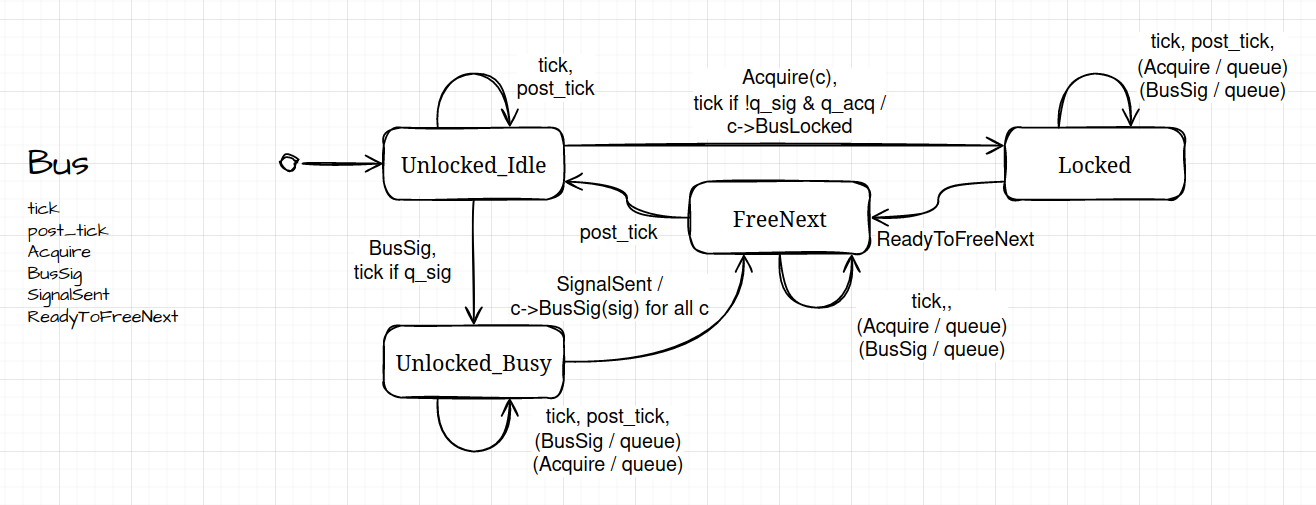
\includegraphics[width=9cm]{img/state_diagram_bus.png}
\textsc{Bus}
\end{center}


\begin{center}
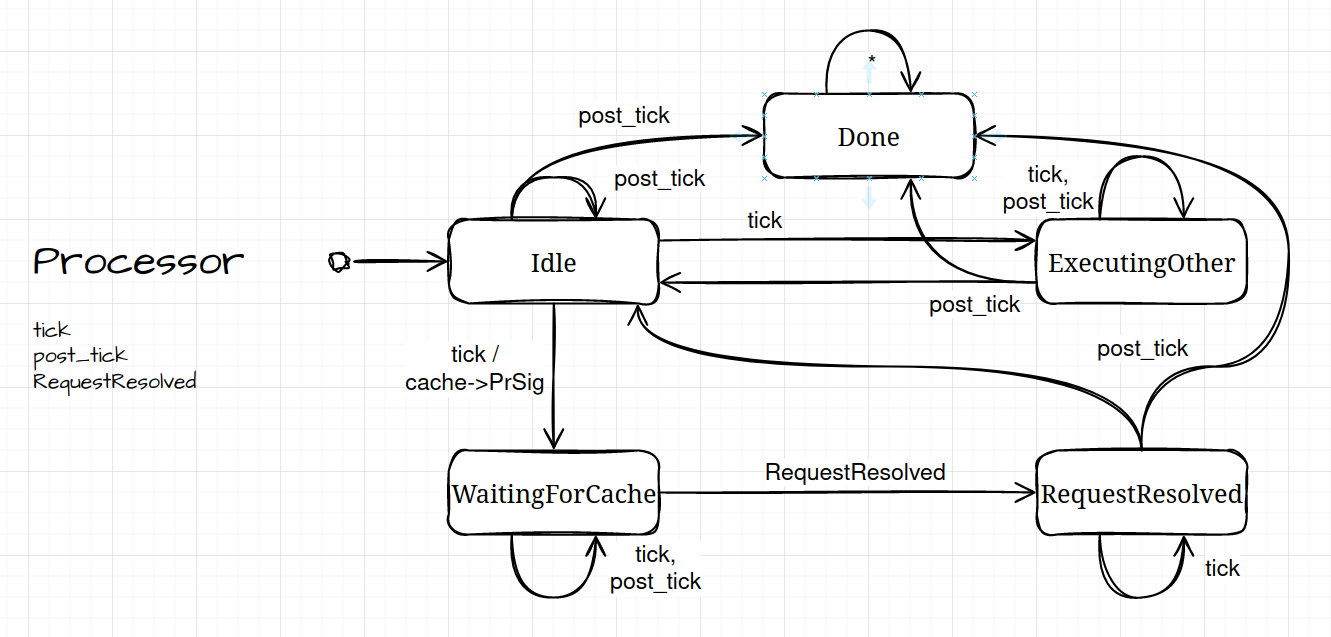
\includegraphics[width=9cm]{img/state_diagram_processor.png}
\textsc{Processors}
\end{center}

\end{multicols}

\begin{center}
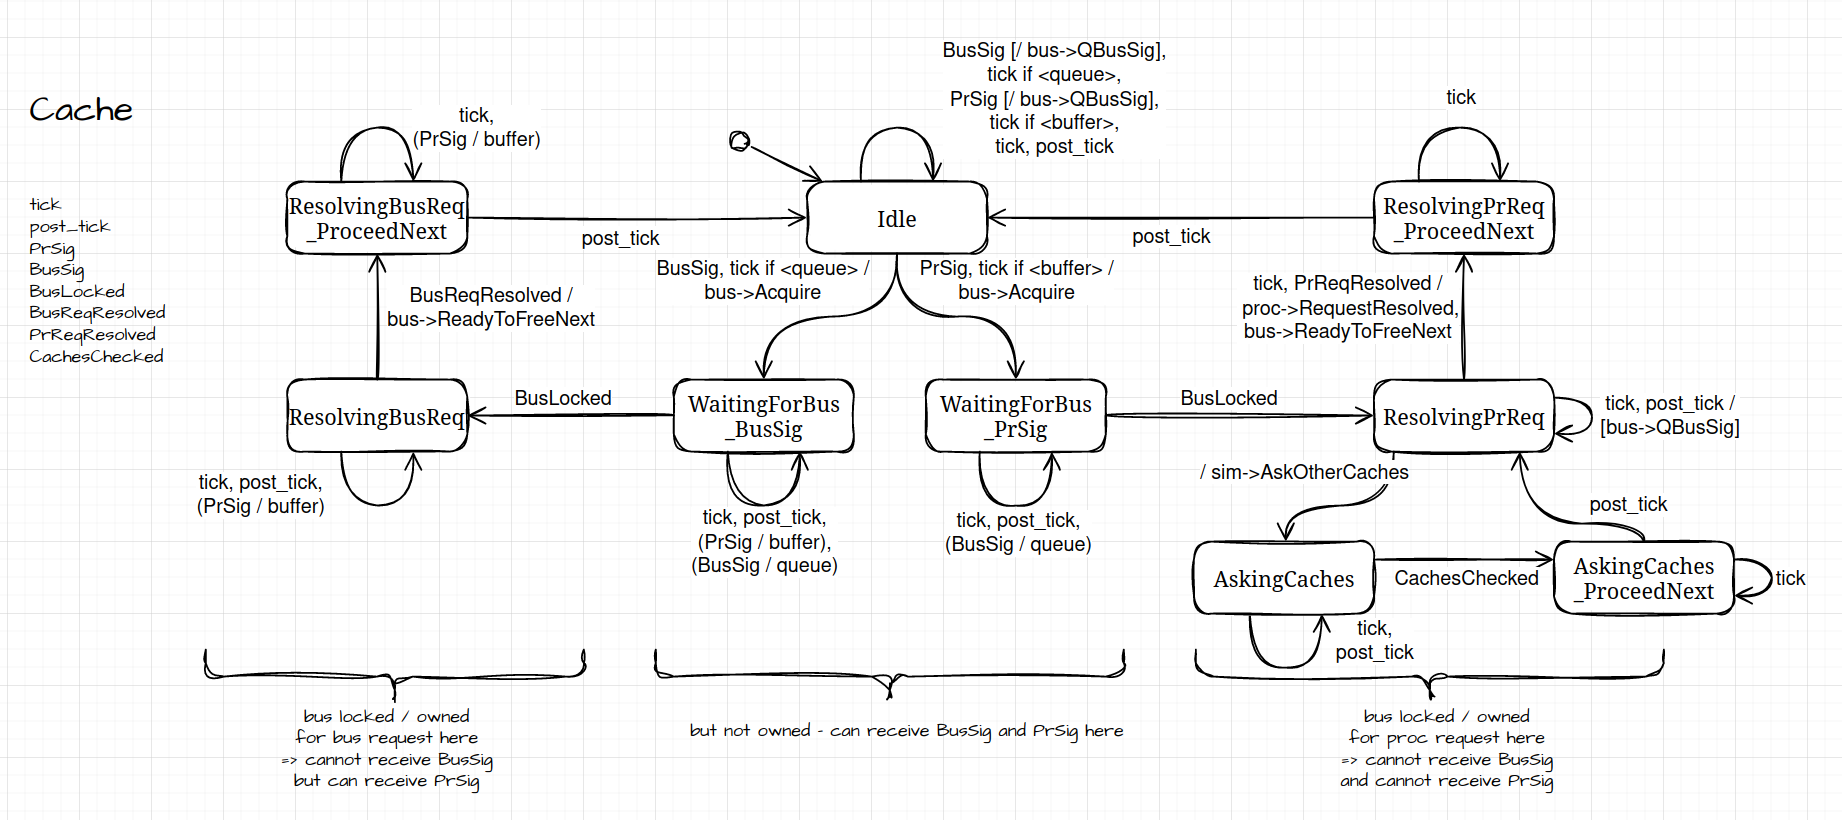
\includegraphics[width=18cm]{img/state_diagram_cache.png}
\textsc{Caches}
\end{center}

\begin{multicols}{2}

\subsubsection{delayed queue}

Building a system of communicating FSMs requires some communication channel. For this purpose, we implemented a new data-structure which is essentially a message queue with a discrete delay. Say a cache needs to send something to its processor, but this process is supposed to take two cycles. With a delayed queue interface, this is amazingly simple:

\begin{code}[Rust]{}
fn some_function() {
    <-- snip -->
    let send_proc = |&self_: Self, msg: ProcMsg, delay: i32| {
        self.tx.send(DelayedMsg {
            t: delay,
            msg: Msg::CacheToProc(proc_id,msg),
        }).unwrap();
    };
    // tx provides the interface for sending to the queue
    send_proc(self, ProcMsg::RequestResolved, 0);
}
\end{code}

The first fully functional implementation was based on a priority queue using binary heap, prioritized by the timestamps/delays of the messages. In an attempt to speed things up, we later re-implemented the same functionality based on a ring-buffered queue which is slower in the worst case, but faster on average than the binary heap. The ring buffer implementation turned out to be faster, especially when enabling the highest level of optimizations in \textit{rustc}.

The amazing support for algebraic data types and pattern matching in Rust keeps the encoding of the state transitions simple. Below you can see how this is done by the example of a part of the message handler of the bus.

\begin{code}[Rust]{Bus MsgHandler}
impl MsgHandler<BusMsg> for Bus<'_> {
    fn handle_msg(&mut self, msg: BusMsg) {
        match self.state {
            <-- see next -->
        }
    }
}
\end{code}

\textit{MsgHandler} is the \textit{trait} (comparable to an \textit{interface} in Java) and \textit{handle\_msg} will be invoked by the simulator when there's a message in the queue with the current cycle as timestamp, addressed at the bus. Based on the bus's current state and the message, it can then trigger state transitions:

\begin{code}[Rust]{Bus MsgHandler continued}
<-- snip -->
BusState::Unlocked_Idle => {
    match msg {
        BusMsg::Tick => {
            // transition
        },
        BusMsg::PostTick => (),
        BusMsg::Acquire(cache_id) => {
            // transition
        },
        BusMsg::BusSig(cache_id, sig) => {
            // transition
        },
        _ => panic!("Invalid bus state"),
    }
},
BusState::Unlocked_Busy => ...
<-- snip -->
\end{code}

\subsubsection{optimizations and accessibility}

The rich type system of Rust already enables quite substantial optimizations at compile time, which can be supported by using generic types etc. The re-implementation of the delayed queue for speed was mentioned in the previous section. It is also worth noting that turning on optimizations in the rust compiler (compiling for \textit{release}) had a substantial impact on performance.

Further, code-based optimizations focused on preventing unnecessary ticks of components in states where a \textit{tick} message cannot cause any progress, which is fairly easy when all components are simply finite state machines and all communication goes through a central message queue.

\begin{code}[Rust]{Simulator Optimizations}
match procs[proc_id as usize].state {
    // some optional optimizations
    ProcState::WaitingForCache | ProcState::Done => continue,
    _ => send_msg(Msg::ToProc(proc_id, Tick)),
};
\end{code}

Furthermore, it is worth noting that this system is - by design - easily parallelizable using multi-threading. However, because of the central message queue, all threads should run on the same core in order to share memory when running the simulation.

We also used the opportunity to do some WebAssembly (\textit{WASM}) benchmarking. We could compile the simulator to WASM architectures without any code changes. The execution time of the WASI version was only about twice that of the native one, which is quite impressive.

\end{multicols}

\section{Analysis}

\subsection{MESI}

\subsection{Dragon}

\end{document}